\section{Resultados Prueba de Vuelo}
\subsection{Análisis de Resultados GPS Controlador de Vuelo}

A continuación, se presenta los resultados obtenidos de la trayectoría GPS del UAV de ala fija. La figura \ref{fig:GPS_pruebaVuelo} muestra el recorrido efectuado por el UAV de ala fija durante la prueba de vuelo, la cual fue realizada por un piloto especializado especializado en el manejo de este tipo de aeronaves. La trayectoria registrada refleja la complejidad del vuelo, donde el piloto ejecutó diversas maniobras y movimientos a lo largo de un periodo prolongado. La capacidad del piloto para controlar el UAV se evidencia en las variaciones y cambios de dirección observados en la imagen. Se resalta el hecho de que en esta imagen no se puede observar adecuadamente como fue el recorrido de la aeronave, ya que hay gran variedad de virajes realizadas por la aeronave. 
\begin{figure}[H]
    \centering
    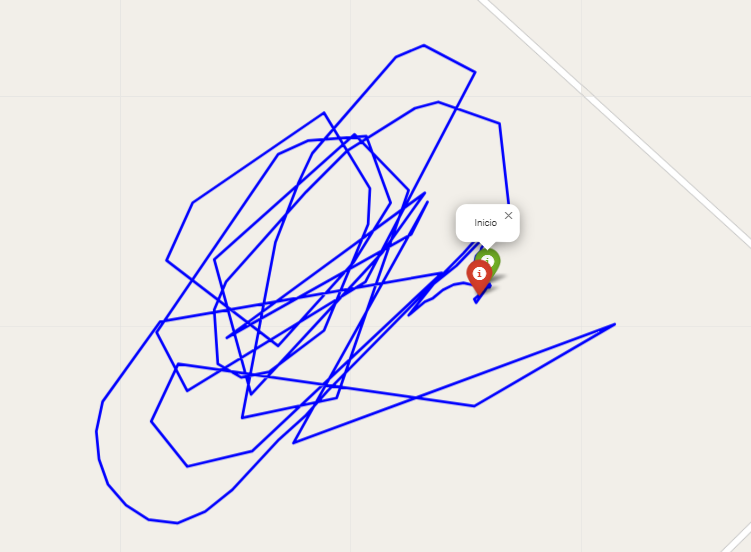
\includegraphics[width=12 cm]{Imagenes/Vuelo/gps_Prueba.png}
    \caption{Recorrido del UAV prueba de Vuelo}
    \label{fig:GPS_pruebaVuelo}
\end{figure}

Seguidamente se realizo una imagen que proporciona una visualización en 3D del movimiento del UAV en relación con su altitud (véase \ref{fig:GPS_altitud}). En esta gráfica, se distinguen claramente las fases de ascenso y descenso del UAV, con diferentes colores para cada fase del vuelo: \\

Ascenso (Azul): La sección marcada en azul muestra el trayecto de ascenso del UAV. Se observa una subida gradual y controlada en la altitud, lo que indica que el piloto pudo manejar eficientemente el aumento de altitud del UAV.\\
Descenso (Verde): La sección marcada en verde indica el trayecto de descenso. Al igual que en el ascenso, el descenso muestra una disminución gradual y controlada en la altitud, lo que sugiere un buen desempeño del piloto en la fase de descenso.


\begin{figure}[H]
    \centering
    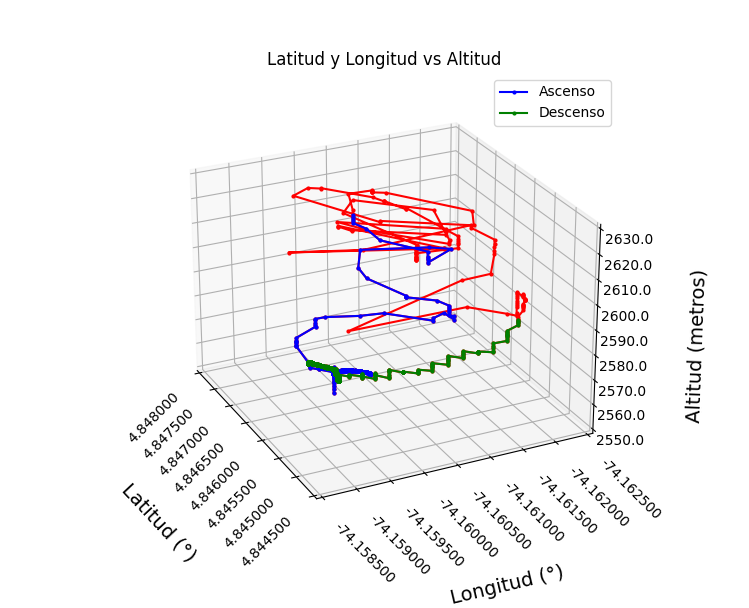
\includegraphics[width=\textwidth]{Imagenes/Vuelo/latitud y longitud acenso.png}
    \caption{Latitud y Longitud vs Altitud}
    \label{fig:GPS_altitud}
\end{figure}


\subsection{Datos Recibidos del Barómetro BMP280 Controlador de Vuelo}
Los datos obtenidos del barómetro BMP280 durante la prueba de vuelo del UAV se pueden observar a continuación (véase \ref{fig:datos obtenidos bmp280}). En donde podemos contrastar altitud, temperatura y presión vs tiempo.\\
\begin{itemize}
    \item \textbf{Altitud vs Tiempo:} Entre aproximadamente 600 y 1150 segundos se realizó la prueba de vuelo, observándose un aumento de altitud de alrededor de 60 metros. A los 1100 segundos se aprecia una bajada progresiva de nivel, que corresponde a las maniobras de descenso del UAV.\\
    \item \textbf{Temperatura vs Tiempo:} La temperatura medida dentro del dispositivo muestra un aumento progresivo durante el periodo de vuelo, reflejando el calentamiento de los componentes internos del UAV.\\
    \item \textbf{Presión vs Tiempo:} La presión atmosférica se mantuvo estable la mayor parte del tiempo, excepto durante el ascenso del UAV, donde se registró una caída significativa, lo que es coherente con el aumento de altitud. Posteriormente, la presión se estabiliza una vez que el UAV alcanza su altitud máxima y durante el descenso.
    
\end{itemize}



\begin{figure}[H]
    \centering
    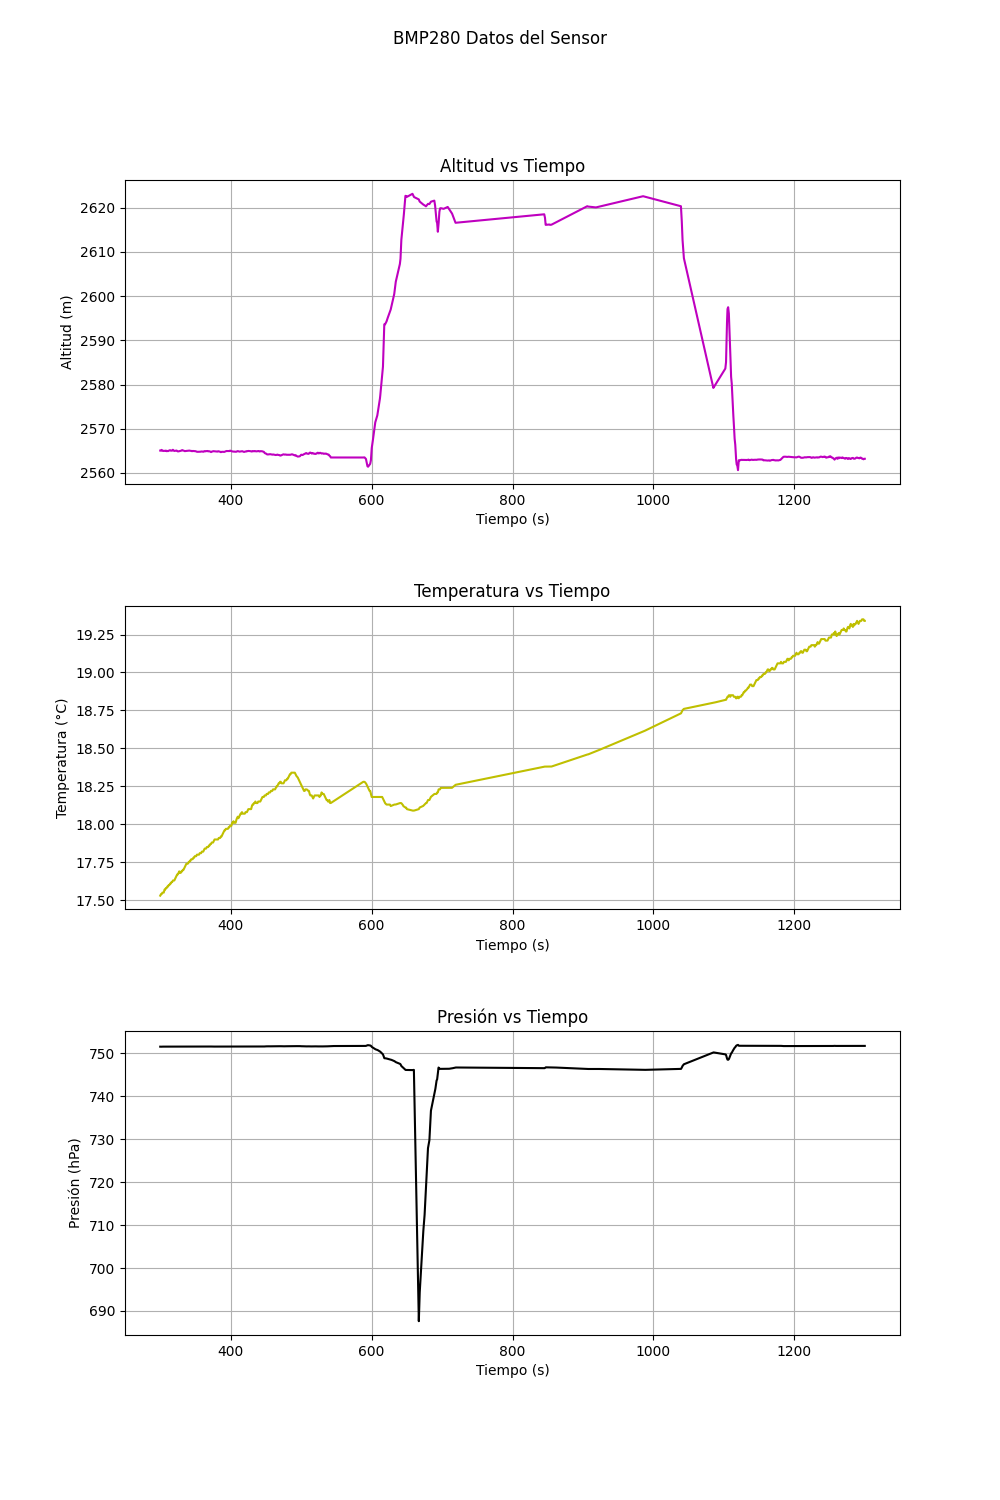
\includegraphics[width=\textwidth]{Imagenes/Vuelo/BMP280_sensor.png}
    \caption{Datos Obtenidos BMP280}
    \label{fig:datos obtenidos bmp280}
\end{figure}



En resumen, los datos indican que el vuelo realizado por el piloto fue exitoso. El incremento en altitud, el comportamiento térmico y las variaciones en la presión atmosférica observadas son coherentes con las expectativas de un vuelo controlado. 


\subsection{Análisis de Resultados de los Ángulos de Movimiento del UAV Controlador de Vuelo}
Datos Recibidos del Sensor BNO055
Los datos de orientación obtenidos del sensor BNO055 durante la prueba de vuelo del UAV.  En las figuras  \ref{fig:datosYawPitch, roll} y \ref{fig:datos obtenidos BNO055} se pueden observar los registros de los ángulos de roll, pitch, yaw y compass a lo largo del tiempo. Estos gráficos muestran cómo el UAV se comportó en términos de orientación durante las diferentes fases del vuelo. \\ 

\begin{itemize}
    \item \textbf{Roll vs Tiempo:} El ángulo de roll varía entre -40 y 80 grados. Estas variaciones son típicas en aeronaves, ya que valores cercanos a 90 grados podrían comprometer la estabilidad del UAV. Los valores observados son comunes en los ángulos de banqueo de la aeronave.\\

    \item \textbf{Pitch vs Tiempo:} El ángulo de pitch varía entre -40 y 40 grados. Estos valores son usuales para evitar que la aeronave entre en situaciones de "pique", lo que podría ser peligroso. Se mantuvo cuidado en esta parte para asegurar la estabilidad del UAV.\\

\item \textbf{Yaw vs Tiempo: }El ángulo de yaw muestra oscilaciones características durante los virajes de la aeronave. Estos cambios abruptos en la orientación están relacionados con los giros efectuados por el piloto.\\

\item \textbf{Compass vs Tiempo:}Similar al yaw, el compás muestra oscilaciones durante los virajes, reflejando los cambios de dirección del UAV. La coincidencia de estos cambios con el roll indica la correlación entre los virajes y el banqueo de la aeronave.
\end{itemize}


\begin{figure}[H]
    \centering
    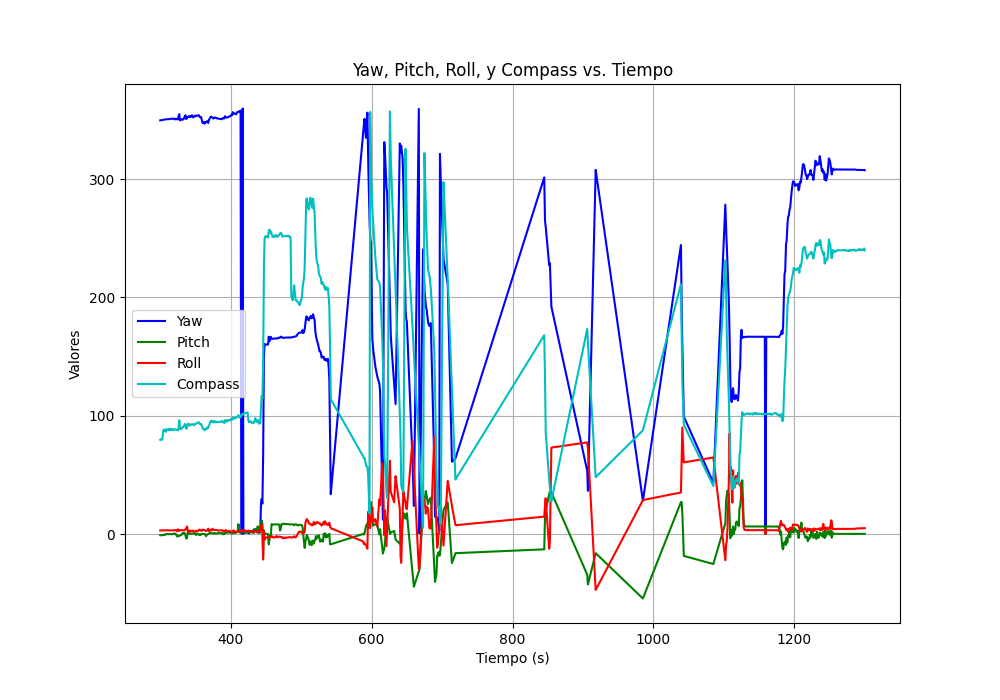
\includegraphics[width=13 cm]{Imagenes/Vuelo/yaw_pitch_roll_vs_tiempo.png}
    \caption{Yaw, Pitch, Roll y Compas vs Tiempo}
    \label{fig:datosYawPitch, roll}
\end{figure}


\begin{figure}[H]
    \centering
    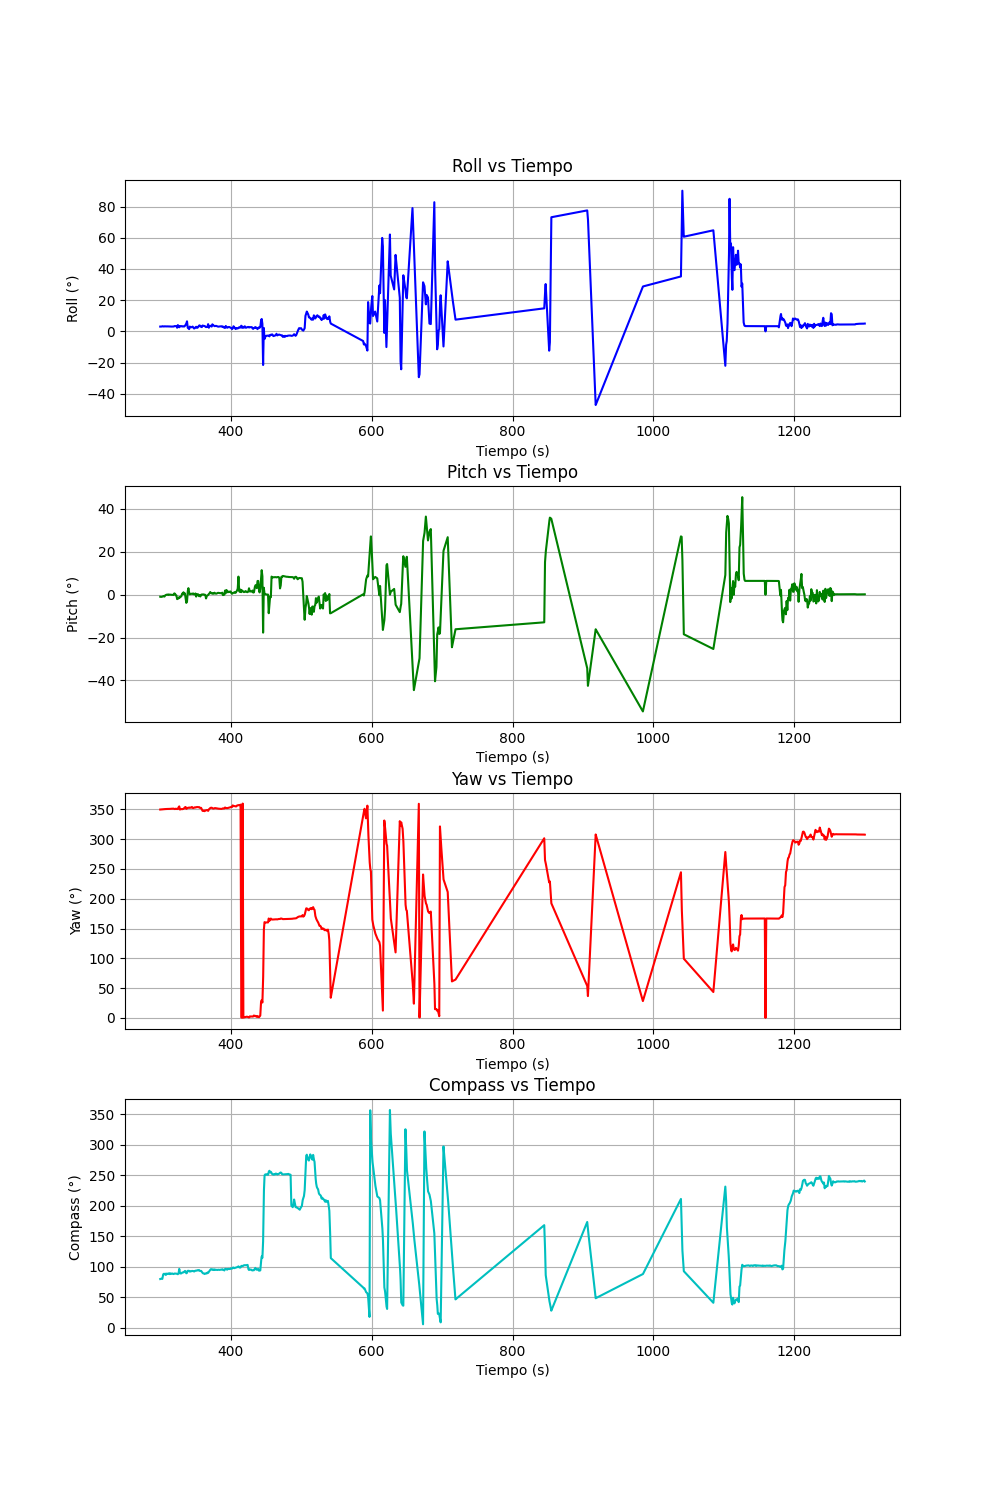
\includegraphics[width=15 cm]{Imagenes/Vuelo/BNO055_orientacion.png}
    \caption{Datos Obtenidos BNO055}
    \label{fig:datos obtenidos BNO055}
\end{figure}


\subsection{Transmisión y Recepción de Datos}

La figura \ref{fig:comparacion transmision y recepcion} muestra los datos transmitidos y recibidos durante la experimentación del vuelo del UAV. Aunque en algunos momentos los datos parecen coincidir, hay varios puntos en los que se observa una considerable pérdida de paquetes y corrupción de datos.\\

En el caso de la altitud, hay un gran desequilibrio entre los datos enviados y recibidos, con diferencias notables que indican transmisiones fallidas. Esto sugiere que hubo errores en la codificación de los datos antes de su transmisión y en la decodificación después de su recepción. Si estos procesos no se realizan correctamente, los datos pueden llegar dañados, justificando la discrepancia observada.\\

Los datos de presión también muestran una gran diferencia entre los valores transmitidos y recibidos. Este problema podría deberse a la pérdida parcial de paquetes durante la transmisión. El módulo nRF24L01, limitado a 32 bits por paquete, puede experimentar pérdidas fraccionarias que afectan severamente la integridad de los datos. La pérdida o corrupción de partes de un paquete puede hacer que los datos recibidos sean muy diferentes de los datos transmitidos.\\

Al observar los puntos obtenidos del GPS, se detecta una pérdida considerable de información transmitida durante el vuelo. Se observan incongruencias en los valores obtenidos, como 21.478790,529.000000, que no es una posición geográfica válida. Además, muchos valores del vuelo no se actualizaron correctamente, lo que sugiere una corrupción y pérdida sustancial de la información.\\

Estas observaciones destacan la necesidad de revisar y mejorar los procesos de codificación y decodificación para asegurar que los datos se transmitan y reciban de manera precisa y coherente, minimizando las pérdidas y corrupciones en futuras pruebas de vuelo del UAV.



\begin{figure}[H]
    \centering
    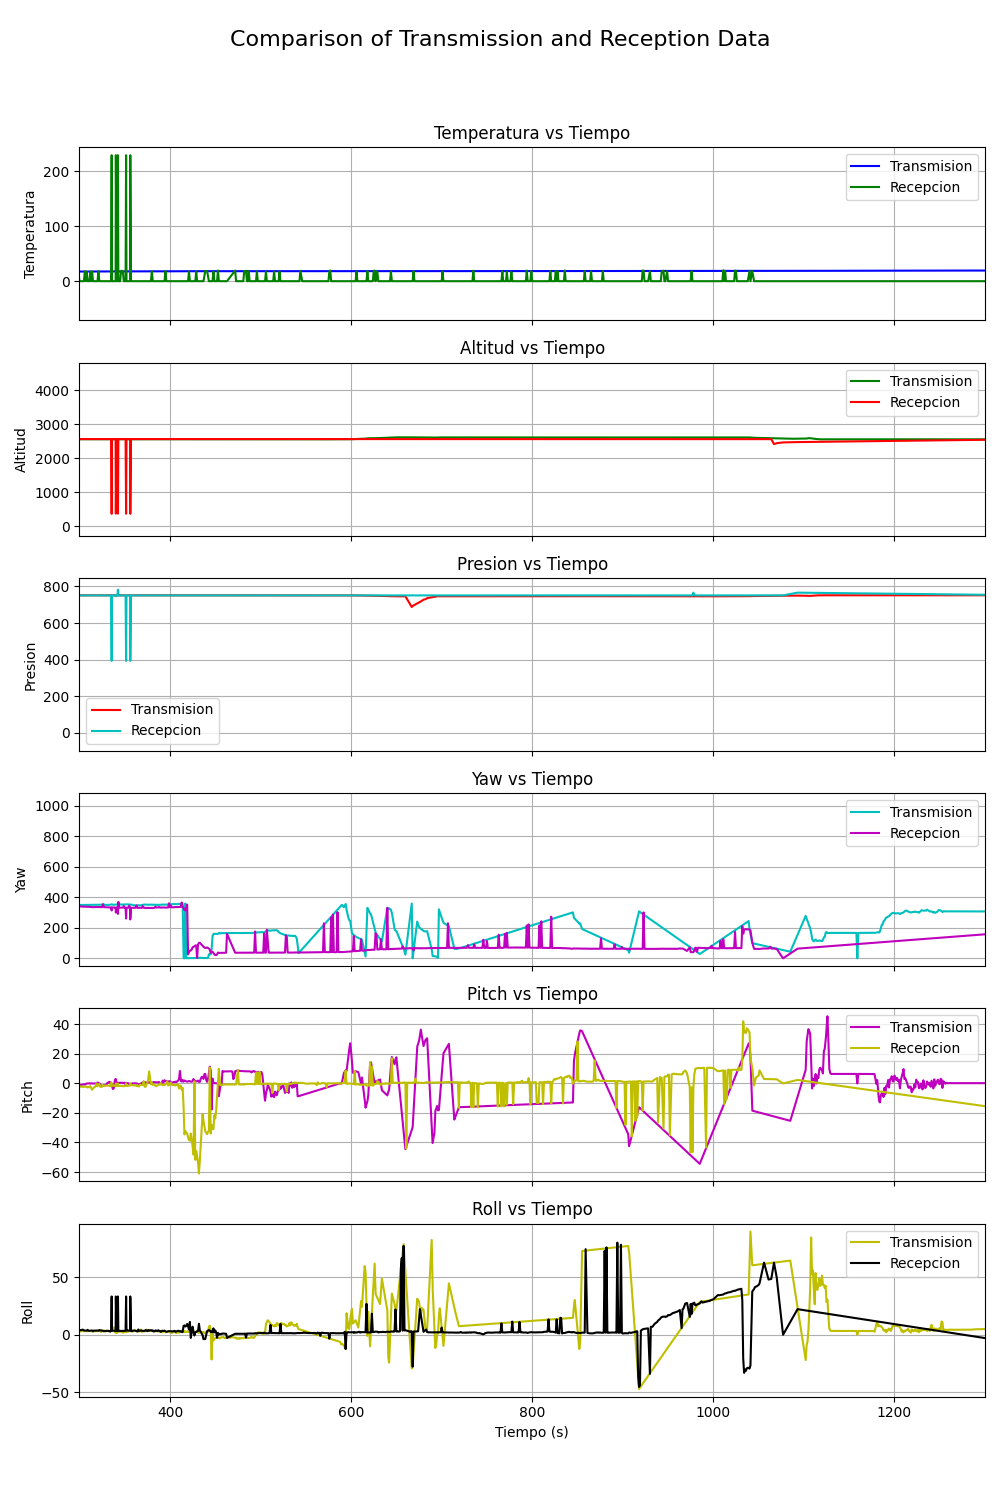
\includegraphics[width=\textwidth]{Imagenes/Vuelo/comparison_subplots.png}
    \caption{Comparación datos Transmisión y Recepción}
    \label{fig:comparacion transmision y recepcion}
\end{figure}

\subsection{Recepción datos de la Interfaz}


La figura  \ref{fig:Datos guardados Interfaz} muestra los datos visualizados por la interfaz de comunicación durante el vuelo del UAV, mostrando al igual que como se hizo anteriormente las variables previamente expuestas. En este grafico, a diferencia de los anteriores se muestran picos y fluctuaciones de las distintas señales. Se hace notable que las señales son representadas con pulsos cuadrados, lo que indica problemas en la recepción de información. \\

Los datos de altitud presentan numerosos picos, sugiriendo interrupciones y pérdidas de paquetes. Esto refleja problemas significativos en la transmisión de esta información. La temperatura muestra inconsistencias similares, con picos abruptos que indican que no se recibió adecuadamente la información. Los datos de presión también tienen grandes fluctuaciones, lo que sugiere problemas en la transmisión y recepción de esta variable. Además, las variables de orientación (yaw, pitch, roll) muestran variaciones bruscas y picos, reflejando inconsistencias y posibles pérdidas de datos durante la transmisión.

\subsubsection{Problemas Identificados}
La transmisión de datos está generando un cuello de botella que afecta la integridad de la información recibida. Esto se debe a la limitación del módulo nRF24L01, que puede experimentar pérdidas de paquetes y corrupción de datos.

\subsubsection{Solución Propuesta}
Para mitigar estos problemas, es esencial implementar un buffer en la interfaz de la comunicación serial. Este buffer almacenará temporalmente los datos antes de su transmisión, permitiendo una mejor gestión del flujo de información y asegurando una transmisión más eficiente. Además, es crucial optimizar la interfaz de usuario para evitar lags y asegurar una fluidez correcta en la visualización de los datos. Esto mejorará la capacidad de monitoreo en tiempo real y la fiabilidad de la información presentada.

\begin{figure}[H]
    \centering
    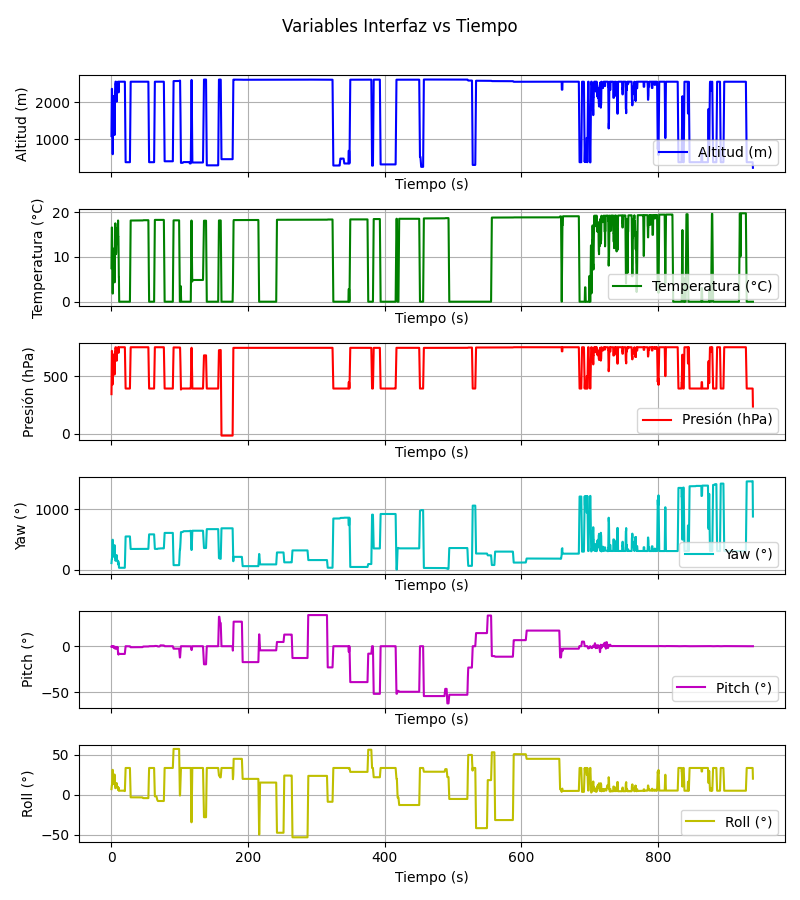
\includegraphics[width=\textwidth]{Imagenes/Vuelo/subplots_interfaz.png}
    \caption{Datos Guardados Interfaz}
    \label{fig:Datos guardados Interfaz}
\end{figure}